\section{Scheduler Flow Control}

As defined by the Kernel's documentation on CFS,

"80\% of CFS's design can be summed up in a single sentence: CFS basically models an 'ideal, precise multi-tasking CPU' on real hardware." [2]
\vspace{1pc}

Looking inside the Kernel source, there are several files of interest that hold particular importance to the development and tuning of the scheduler.

\begin{description}
	\item[Kernel/sched/sched.h] contains numerous preprocessor definitions, function prototypes, constants for use in weighting and organizing processes.
	\item[Kernel/sched/core.c] handles the primary scheduling overhead including the main schedule() function, and manages multiple scheduling policies and run queues.
	\item[Kernel/sched/fair.c] defines nearly all CFS behaviors and rules (such as picking the next task to run), defines constants specific to CFS, and includes structs such as fair\_sched\_class.
	\item[lib/rbtree.c] contains the class definition for the red-black tree system used by CFS, and includes functions for quickly navigating between adjacent nodes in the tree as well as finding the leftmost node (which is typically the most critical process to run).
	\item[include/linux/sched/prio.h] holds several priority constants including minimum and maximum niceness values, and the default values for newly created processes
	\item[include/linux/sched/rt.h] contains, among other things, the Round Robin timeslice multiplier for SCHED\_RR which directly impacts the system's final default Round Robin timeslice.
\end{description}

Digging deeper into each of these files revealed some particular areas of interest for modifying scheduling behavior. \textbf{Core.c} holds the primary overhead control on scheduling in the Kernel which makes it a prime candidate to start exploring. Core.c's primary function is \texttt{Schedule()} which handles scheduling flow control between runqueues such as the CFS runqueue. \texttt{Schedule()} calls can be triggered by blocking from Mutexes, Semephores and several other elements and it is capable of handling both realtime scheduling policies (Round Robin, FIFO) and non-preemptable policies (Batch).

Schedule() makes a call to \texttt{pick\_next\_task(rq, prev)}, where rq represents the active runqueue and prev represents the current task\_struct being executed. \texttt{Pick\_next\_task()} then passes control to the appropriate scheduler class (such as CFS) where the scheduler class will run its own implementation of \texttt{pick\_next\_task()}. When CFS is the current scheduling class, \texttt{fair\_sched\_class.pick\_next\_task(rq, prev)} is called, sending control to fair.c's function \texttt{pick\_next\_task\_fair(rq,prev)}.

\texttt{pick\_next\_task\_fair()} contains a variety of additional rules, regulations and exceptions for choosing tasks. \texttt{pick\_next\_task\_fair()} will return the task\_struct of the process it selects to run next to core.c and, in the event that the CFS chooses to run the idle process, it will return \texttt{NULL}.

Under the "Simple" clause of this function, \texttt{pick\_next\_entity(cfs\_rq, sched\_entity)} is called, where the leftmost node of the red-black tree of tasks is chosen unless overridden to re-run the last process or run the skip buddy. This is effectively the method where processes are actually chosen in the CFS scheduler.


\begin{figure}[hb]
	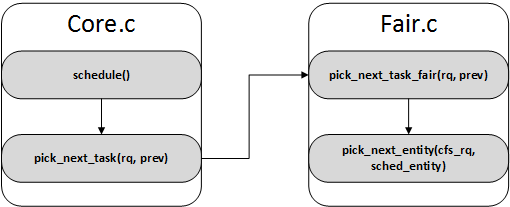
\includegraphics[width=1.0\columnwidth]{images/flowcontrol}
	\caption{Simplified version of the scheduler's flow control}
\end{figure}
